\chapter{The Large Hadron Collider and the ATLAS Detector}

\section{The Large Hadron Collider}

The Large Hadron Collider (LHC), located at CERN near Geneva, Switzerland, is currently the world's largest and most
powerful particle accelerator. It was designed to facilitate high-energy proton-proton and heavy-ion collisions with the
objective of probing the fundamental structure of the universe.

The LHC, a 27 km circumference ring situated 100 meters underground, operates by accelerating two beams of protons to
near the speed of light in opposite directions. These beams are then steered into collision at four interaction points
where the LHC's main experiments, ATLAS, CMS, ALICE, and LHCb, are situated.

\section{The ATLAS Detector}

The ATLAS (A Toroidal LHC ApparatuS) detector, one of the two general-purpose detectors at the LHC, is designed to
measure a broad range of particles and phenomena produced in the LHC's proton-proton collisions. With a length of 44
meters and a diameter of 25 meters, it's a massive instrument consisting of several layers each dedicated to detecting
different types of particles.

From innermost to outermost, the main components of the ATLAS detector are the Inner Detector for tracking, the
Electromagnetic and Hadronic Calorimeters for energy measurements, and the Muon Spectrometer for detecting muons.
Surrounding the entire apparatus is a complex magnet system that bends the trajectories of charged particles, allowing
for the determination of their momentum.

\section{Data Acquisition and Processing}

When proton-proton collisions occur in the ATLAS detector, the produced particles traverse the detector layers, leaving
behind signals that are transformed into digital data. Given the LHC's high collision rate, it's crucial to select only
the potentially interesting events for further analysis, a task performed by the ATLAS trigger system.

The trigger system operates in several levels, with each level applying increasingly precise selection criteria to
reduce the data rate. After passing the trigger system, the selected collision events are stored for offline analysis.

The raw data then undergoes a processing stage known as reconstruction. This process translates the raw detector signals
into identifiable physics objects such as electrons, muons, photons, and jets.

\section{Data Analysis and Event Selection}

The primary objective of data analysis in particle physics is to extract interesting physics events from a vast amount
of collected data. The initial stage of data analysis involves event selection, where specific criteria are applied to
separate potential signal events from background noise.

In the context of our ttH analysis in the 2lSS1Tau channel, event selection criteria include the identification of two
same-sign leptons and one hadronically decaying tau lepton. Moreover, additional conditions may be applied to identify
the presence of jets, especially b-jets, which are indicative of top quark decay.

However, even with strict event selection criteria, a significant number of background events can mimic the ttH signal.
The most common background processes include ttW and ttZ events, Drell-Yan events, and others. These backgrounds are
estimated using a combination of data-driven methods and Monte Carlo simulations and are subtracted from the observed
data to reveal the potential ttH signal.

\section{Simulated Data and Event Weighting}

Simulated data plays a critical role in particle physics experiments. To interpret the experimental results, we need to
understand what we would expect to observe under different theoretical models. This is accomplished through detailed
simulations of the processes of interest, as well as the response of the detector to these processes.

Monte Carlo (MC) methods are commonly used for these simulations. The MC simulation provides a probabilistic
interpretation of the quantum mechanical processes that occur during particle collisions, as well as the subsequent
decay and detection of the produced particles. However, MC simulations start from an idealized condition, assuming
perfect detector operation and ignoring many real-world factors that can affect the data.

To align the MC simulated data with the real data, it is necessary to apply event weights. Event weighting is a
technique used to correct the simulated distributions for known differences between the simulation and the real data.

Event weights can account for a variety of effects:

Luminosity: The total number of simulated events often does not correspond to the luminosity of the real data. Events
are therefore weighted to correspond to the correct integrated luminosity. If $L_{data}$ is the integrated luminosity of
the data and $L_{MC}$ is the integrated luminosity of the MC sample, then the luminosity weight for an event is $w_{L} =
    L_{data}/L_{MC}$.

Cross-Section: Different processes have different probabilities (cross-sections) of occurring. The ratio of the
cross-sections in data and simulation $\sigma_{data}/\sigma_{MC}$ is used as a weight.

Detector Effects: The detector response is not always perfectly simulated. Therefore, weights are applied to correct for
known discrepancies in detector efficiencies and energy resolutions between the data and the simulation.

Pileup: Pileup refers to additional proton-proton collisions that occur simultaneously with the event of interest.
Pileup can significantly affect the event reconstruction. Pileup weights are used to match the pileup distribution in
the data.

Higher-order corrections: Theoretical predictions often include higher-order corrections, known as K-factors, to account
for processes beyond the leading-order approximation used in the simulation.

In mathematical terms, the total weight $w_{total}$ for an event can be written as the product of individual weights:

\begin{equation}
    w_{\text{total}} = w_{L} w_{\sigma} w_{\text{detector}} w_{\text{pileup}} w_{\text{K-factor}}
\end{equation}

Event weights are essential for ensuring that the simulated events accurately represent the conditions of the actual
experiment. These weights allow us to make meaningful comparisons between the data and theoretical predictions, and are
a crucial part of the analysis in high-energy physics.


\section{V8 adaptation}

\section{\gls{sr} cut expression}
\label{appendix:cut-expression}

{\scriptsize
    \begin{verbatim}
    custTrigMatch_LooseID_FCLooseIso_DLT
    && (dilep_type && (lep_ID_0*lep_ID_1)>0)
    && ((lep_Pt_0 >= 10e3 && lep_Pt_1 >= 10e3) && (fabs(lep_Eta_0) <= 2.5 && fabs(lep_Eta_1) <= 2.5)
        && ((abs(lep_ID_0) == 13 && lep_isMedium_0 && lep_isolationLoose_VarRad_0 && passPLIVTight_0)
            || ((abs(lep_ID_0) == 11 && lep_isTightLH_0 && lep_isolationLoose_VarRad_0 && passPLIVTight_0
                && lep_ambiguityType_0 == 0 && lep_chargeIDBDTResult_recalc_rel207_tight_0 > 0.7)
                && ((!(!(lep_Mtrktrk_atConvV_CO_0 < 0.1 && lep_Mtrktrk_atConvV_CO_0 >= 0 && lep_RadiusCO_0 > 20)
                    && (lep_Mtrktrk_atPV_CO_0 < 0.1 && lep_Mtrktrk_atPV_CO_0 >= 0)))
                    && !(lep_Mtrktrk_atConvV_CO_0 <0.1 && lep_Mtrktrk_atConvV_CO_0 >= 0 && lep_RadiusCO_0 > 20))))
            && ((abs(lep_ID_1) == 13 && lep_isMedium_1 && lep_isolationLoose_VarRad_1 && passPLIVTight_1)
                || ((abs(lep_ID_1) == 11 && lep_isTightLH_1 && lep_isolationLoose_VarRad_1 && passPLIVTight_1
                    && lep_ambiguityType_1 == 0 && lep_chargeIDBDTResult_recalc_rel207_tight_1 > 0.7)
                    && ((!(!(lep_Mtrktrk_atConvV_CO_1 < 0.1 && lep_Mtrktrk_atConvV_CO_1 >= 0 && lep_RadiusCO_1 > 20)
                        && (lep_Mtrktrk_atPV_CO_1 < 0.1 && lep_Mtrktrk_atPV_CO_1 >= 0)))
                        && !(lep_Mtrktrk_atConvV_CO_1 < 0.1 && lep_Mtrktrk_atConvV_CO_1 >= 0 && lep_RadiusCO_1 > 20)))))
    && nTaus_OR==1
    && nJets_OR_DL1r_85>=1
    && nJets_OR>=4
    && ((dilep_type==2) || abs(Mll01-91.2e3)>10e3)
\end{verbatim}
}

We have kept the cuts the same as \cite{severin}, except for the cut on the \verb|nJets_OR| to \verb|>=4| to keep
consistent definition \gls{sr} definition across the group \todo{refer to the BDT group - how?}.

\section{Yields Plots}
\label{appendix:yields}

\begin{figure}[htb!]
    \centering
    \begin{subfigure}{0.45\textwidth}
        \includegraphics[width=\linewidth]{figures/yields/lep-pt-0.pdf}
        \caption{Distribution of the transverse momentum of the leading lepton.}
    \end{subfigure}\hfill%
    \begin{subfigure}{0.45\textwidth}
        \includegraphics[width=\linewidth]{figures/yields/lep-pt-1.pdf}
        \caption{Distribution of the transverse momentum of the subleading lepton.}
    \end{subfigure}
\end{figure}

\begin{figure}[htb!]
    \centering
    \begin{subfigure}{0.45\textwidth}
        \includegraphics[width=\linewidth]{figures/yields/n-jets.pdf}
        \caption{Distribution of the number of jets.}
    \end{subfigure}\hfill%
    \begin{subfigure}{0.45\textwidth}
        \includegraphics[width=\linewidth]{figures/yields/n-bjets.pdf}
        \caption{Distribution of the number of $b$-jets.}
    \end{subfigure}
\end{figure}

\begin{figure}[htb!]
    \centering
    \begin{subfigure}{0.45\textwidth}
        \includegraphics[width=\linewidth]{figures/yields/tau-width.pdf}
        \caption{Distribution of the $\tau$-jet width.}
    \end{subfigure}\hfill%
\end{figure}
\subsection{List of samples by each process}

The root directory for the files is:

{\small
\verb|/eos/atlas/atlascerngroupdisk/phys-higgs/HSG8/multilepton_ttWttH/v08/v0801/systematics-full/nominal|
}

The list of samples is given in \hyperref[tab:samples]{Table~\ref*{tab:samples}}.

\newpage

\begin{table}[h!]
    \centering
    \renewcommand{\arraystretch}{1.5}
    \caption{List of samples by each process}
    \label{tab:samples}
    \begin{tabular}{p{1.5cm}p{13.5cm}}
        \toprule
        Process      & \gls{dsid}                                                           \\
        \midrule
        $t\bar{t}H$  & p4498/346343, p4498/346344, p4498/346345                             \\
        $t\bar{t}W$  & p4416/700168, p4590/700205                                           \\
        $t\bar{t}Z$  & p4416/700168                                                         \\
        $t\bar{t}$   & p4308/410470                                                         \\
        $VV$         & p4416/364250, p4416/364253, p4416/364254, p4416/364255, p4308/364283, p4308/364284, p4308/364285,
p4308/364286, p4308/364287, p4308/363355, p4308/363356, p4308/363357, p4308/363358, p4308/363359,
p4308/363360, p4308/363489                                               \\
        $ggVV$       & p4308/345705, p4396/345706, p4396/345715, p4396/345718, p4396/345723 \\
        $Zjets$      & p4308/364100, p4308/364101, p4308/364102, p4308/364103, p4308/364104, p4308/364105, p4308/364106,
p4308/364107, p4308/364108, p4308/364109, p4308/364110, p4308/364111, p4308/364112, p4308/364113,
p4308/364114, p4308/364115, p4308/364116, p4308/364117, p4308/364118, p4308/364119, p4308/364120,
p4308/364121, p4308/364122, p4308/364123, p4308/364124, p4308/364125, p4308/364126, p4308/364127,
p4308/364128, p4308/364129, p4308/364130, p4308/364131, p4308/364132, p4308/364133, p4308/364134,
p4308/364135, p4308/364136, p4308/364137, p4308/364138, p4308/364139, p4308/364140, p4308/364141,
p4308/364198, p4308/364199, p4308/364200, p4308/364201, p4308/364202, p4308/364203, p4308/364204,
p4308/364205, p4308/364206, p4308/364207, p4308/364208, p4308/364209, p4308/364210, p4308/364211,
p4308/364212, p4308/364213, p4308/364214, p4308/364215                                            \\
        $Wjets$      & p4308/364156, p4308/364157, p4308/364158, p4308/364159, p4308/364160, p4308/364161, p4308/364162,
p4308/364163, p4308/364164, p4308/364165, p4308/364166, p4308/364167, p4308/364168, p4308/364169,
p4308/364170, p4308/364171, p4308/364172, p4308/364173, p4308/364174, p4308/364175, p4308/364176,
p4308/364177, p4308/364178, p4308/364179, p4308/364180, p4308/364181, p4308/364182, p4308/364183,
p4308/364184, p4308/364185, p4308/364186, p4308/364187, p4308/364188, p4308/364189, p4308/364190,
p4308/364191, p4308/364192, p4308/364193, p4308/364194, p4308/364195, p4308/364196, p4308/364197                                            \\
        $tW$         & p4308/410646, p4308/410647                                           \\
        $threeTop$   & p4308/304014                                                         \\
        $fourTop$    & p4308/410080                                                         \\
        $t\bar{t}WW$ & p4308/410081                                                         \\
        $tZ$         & p4308/410560                                                         \\
        $WtZ$        & p4308/410408                                                         \\
        $VVV$        & p4308/364242, p4308/364243, p4308/364244, p4308/364245, p4308/364246, p4308/364247, p4308/364248, p4308/364249                                              \\
        $VH$         & p4308/342284, p4308/342285                                           \\
        $tHjb$       & p4308/346799\_AF                                                     \\
        $tWH$        & p4308/346678\_AF                                                     \\
        \bottomrule
    \end{tabular}
\end{table}

\newpage
\subsection{Distribution of the variables inside \gls{sr}}

The following figures (\autoref{fig:distributions1} and \autoref{fig:distributions2}) show the distributions of some variables
of interest inside \gls{sr}.

\captionsetup[subfigure]{justification=centering}
\begin{figure}[htb!]
    \centering
    \begin{subfigure}{0.45\textwidth}
        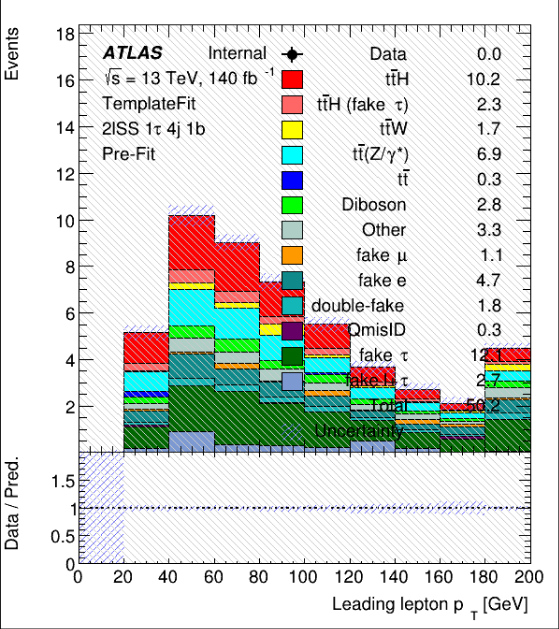
\includegraphics[width=\linewidth]{figures/plots/histograms/lep_pt_0.png}
        \caption{Distribution of the transverse momentum of the leading lepton.}
        \label{fig:lep_pt_0}
    \end{subfigure}\hfill%
    \begin{subfigure}{0.45\textwidth}
        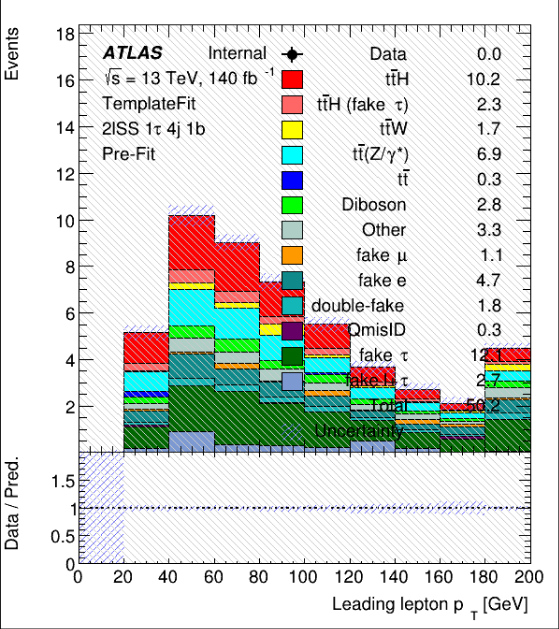
\includegraphics[width=\linewidth]{figures/plots/histograms/lep_pt_1.png}
        \caption{Distribution of the transverse momentum of the subleading lepton.}
        \label{fig:lep_pt_1}
    \end{subfigure}

    \vspace{0.5cm}

    \begin{subfigure}{0.45\textwidth}
        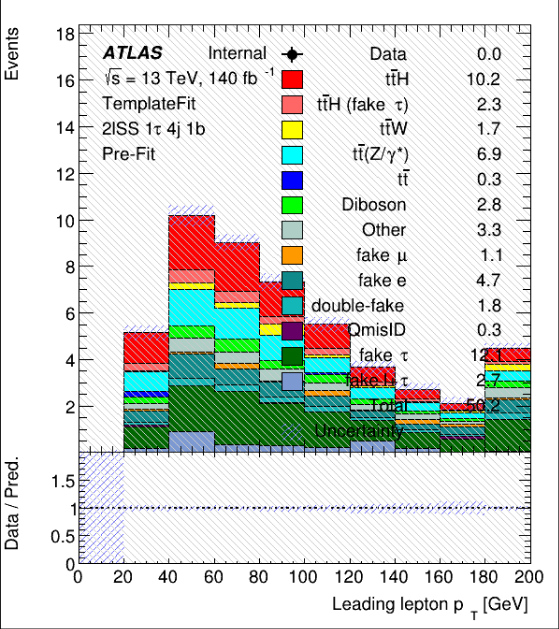
\includegraphics[width=\linewidth]{figures/plots/histograms/lep_Eta_0.png}
        \caption{Distribution of the pseudorapidity of the leading lepton.}
        \label{fig:lep_Eta_0}
    \end{subfigure}\hfill%
    \begin{subfigure}{0.45\textwidth}
        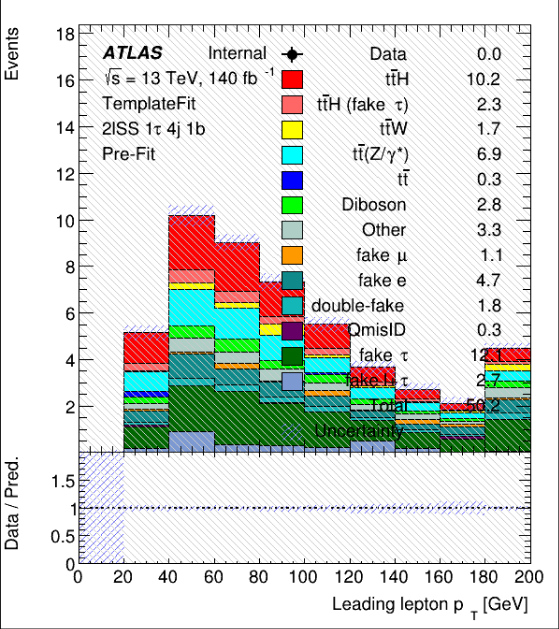
\includegraphics[width=\linewidth]{figures/plots/histograms/lep_Eta_1.png}
        \caption{Distribution of the pseudorapidity of the subleading lepton.}
        \label{fig:lep_Eta_1}
    \end{subfigure}
    \caption{Distributions of the variables inside \gls{sr} (part 1)}
    \label{fig:distributions1}
\end{figure}

\newpage

\begin{figure}[htb!]
    \centering
    \begin{subfigure}{0.45\textwidth}
        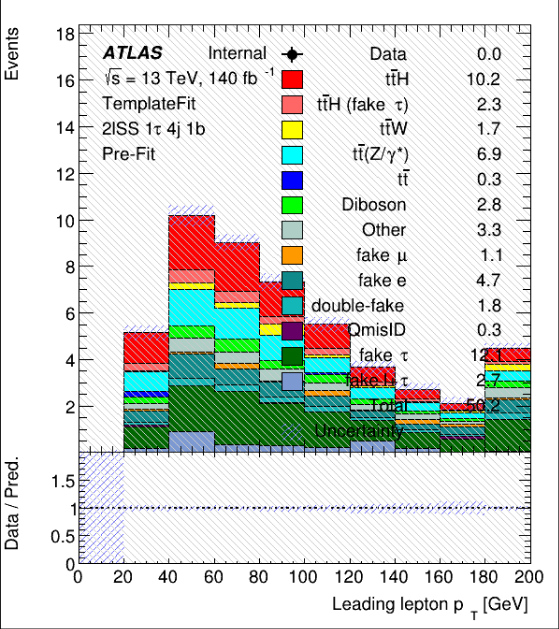
\includegraphics[width=\linewidth]{figures/plots/histograms/lep_Phi_0.png}
        \caption{Distribution of the azimuthal angle of the leading lepton.}
        \label{fig:lep_Phi_0}
    \end{subfigure}\hfill%
    \begin{subfigure}{0.45\textwidth}
        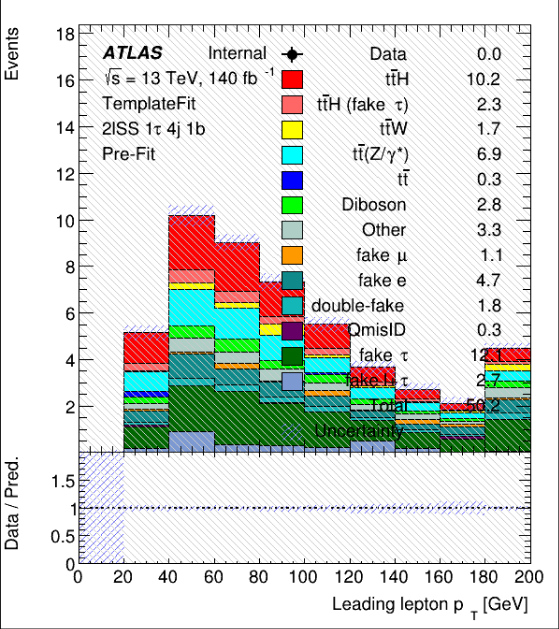
\includegraphics[width=\linewidth]{figures/plots/histograms/lep_Phi_1.png}
        \caption{Distribution of the azimuthal angle of the subleading lepton.}
        \label{fig:lep_Phi_1}
    \end{subfigure}

    \vspace{0.5cm}

    \begin{subfigure}{0.45\textwidth}
        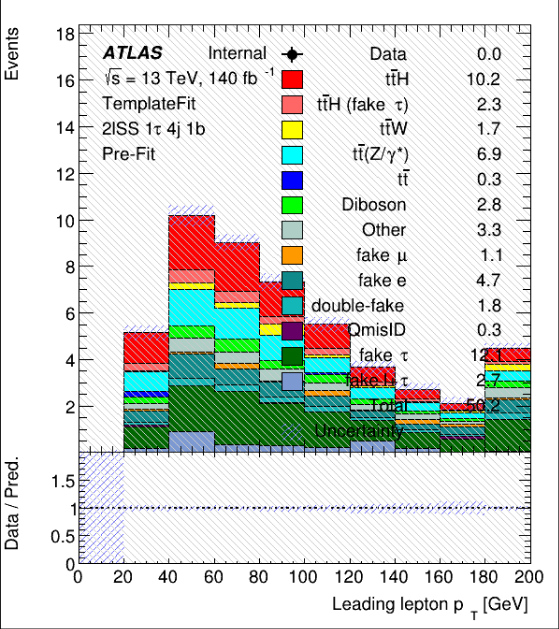
\includegraphics[width=\linewidth]{figures/plots/histograms/njets.png}
        \caption{Distribution of the number of jets.}
        \label{fig:njets}
    \end{subfigure}\hfill%
    \begin{subfigure}{0.45\textwidth}
        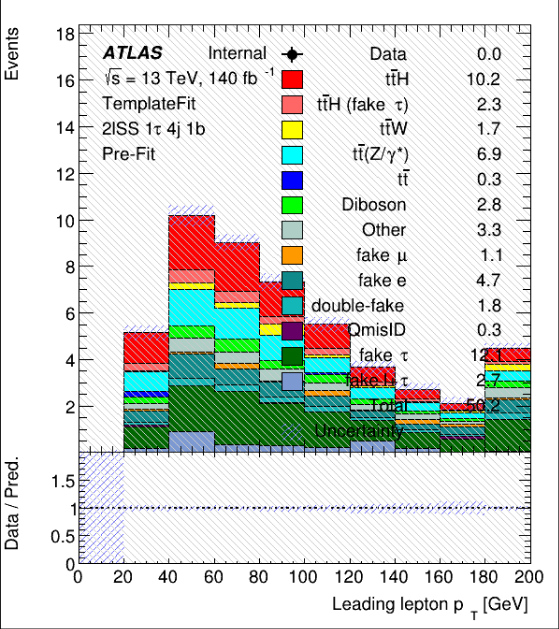
\includegraphics[width=\linewidth]{figures/plots/histograms/nbjets.png}
        \caption{Distribution of the number of $b$-jets.}
        \label{fig:nbjets}
    \end{subfigure}
    \caption{Distributions of the variables inside \gls{sr} (part 2)}
    \label{fig:distributions2}
\end{figure}

\begin{minipage}{0.45\textwidth}
    \centering
    \begin{tabular}{c|c|c|c|c}
        $t\bar{t}H$ & \textbf{v6} & \textbf{v8} &      &       \\
        \hline
        Weighted    & 1000        & 500         & -500 & -50\% \\
        Raw         & 1000        & 500         & -500 & -50\% \\
        \hline
    \end{tabular}
    \captionof{table}{Number of ttH events in the SR for v6 and v8.}
    \label{tab:ttH_event_numbers1}
\end{minipage}\hfill%
\begin{minipage}{0.45\textwidth}
    \centering
    \begin{tabular}{c|c|c|c|c}
        \gls{sr} & \textbf{v6} & \textbf{v8} &      &       \\
        \hline
        Weighted & 1000        & 500         & -500 & -50\% \\
        Raw      & 1000        & 500         & -500 & -50\% \\
        \hline
    \end{tabular}
    \captionof{table}{Number of all the events in the SR for v6 and v8.}
    \label{tab:ttH_event_numbers2}
\end{minipage}

\clearpage \subsection{Features used}

\subsubsection{\texttt{lep\_E\_X}} The energy of the Xth lepton.

\subsubsection{\texttt{DRjj\_lead}} $\Delta R$ between the two leading jets. $\Delta R$ is a distance metric in the
$\eta-\phi$ space frequently used in particle physics.

\subsubsection{\texttt{Ptll01}} The transverse momentum of the dilepton system made up of the two leading leptons.

\subsubsection{\texttt{lep\_nTrackParticles\_X}} The number of track particles associated with the Xth lepton.

\subsubsection{\texttt{custTrigMatch\_LooseID\_FCLooseIso\_DLT}} Custom trigger matching for loosely identified and loosely
isolated leptons, likely related to the dilepton trigger

\subsubsection{\texttt{Mll01}} The invariant mass of the two leading leptons.

\subsubsection{\texttt{Mlll012}} The invariant mass of the three leading leptons.

\subsubsection{\texttt{total\_charge}} The sum of the electric charges of the particles in the event.

\subsubsection{\texttt{HT}} The scalar sum of the transverse momenta of all jets in the event.

\subsubsection{\texttt{HT\_lep}} The scalar sum of the transverse momenta of all leptons in the event.

\subsubsection{\texttt{lep\_Eta\_X}} The pseudorapidity of the Xth lepton.

\subsubsection{\texttt{nTaus\_OR\_Pt25}} The number of overlapping-removed taus with a transverse momentum above 25 GeV.

\subsubsection{\texttt{nFwdJets\_OR}} The number of overlapping-removed forward jets.

\subsubsection{\texttt{MLepMet}} The invariant mass of a lepton and the missing transverse energy vector.

\subsubsection{\texttt{taus\_DL1r\_X}} The DL1r score for the Xth tau.

\subsubsection{\texttt{lep\_isolationLoose\_VarRad\_X}} Indicates whether a lepton (where X refers to the lepton index)
passes an isolation cut with a variable radius. Looser isolation cuts allow more nearby activity in the detector.

\subsubsection{\texttt{lep\_EtaBE2\_X}} The pseudorapidity of the Xth lepton in the second layer of the electromagnetic
calorimeter.

\subsubsection{\texttt{HT\_fwdJets}} The scalar sum of the transverse momenta of all forward jets in the event.

\subsubsection{\texttt{taus\_width\_X}} The width of the Xth tau.

\subsubsection{\texttt{nJets\_OR\_DL1r\_85}} Count of jets that pass overlap removal (OR) and are b-tagged according to the
DL1r algorithm at the 85\% working point.

\subsubsection{\texttt{lep\_nInnerPix\_X}} Number of hits in the inner pixel detector associated with the lepton, where X
refers to the lepton index.

\subsubsection{\texttt{met\_phi}} The azimuthal angle of the missing transverse energy in the event.

\subsubsection{\texttt{DeltaR\_max\_lep\_bjet77}} The maximum DeltaR value between a lepton and a b-tagged jet. The "77"
may refer to the working point of the b-tagging algorithm.

\subsubsection{\texttt{MbX}} Invariant mass associated with the leading b-jet in the event

\subsubsection{\texttt{lep\_RadiusCO\_X}} Possibly the radius of the cone used for isolation of the lepton, or
alternatively a parameter associated with the trajectory of the lepton.

\subsubsection{\texttt{lep\_Mtrktrk\_atConvV\_CO\_X}} The invariant mass of track pairs at the conversion vertex for lepton
X. This might be related to photon conversions into an electron-positron pair.

\subsubsection{\texttt{lep\_Z0SinTheta\_X}} The z0 impact parameter times the sine of the lepton's polar angle.

\subsubsection{\texttt{lep\_Pt\_X}} The transverse momentum of the Xth lepton.

\subsubsection{\texttt{mjjMax\_frwdJet}} The maximum invariant mass of a pair of forward jets.

\subsubsection{\texttt{dilep\_type}} The type of dilepton event (e.g., $ee$, $\mu e$, $\mu \mu$).

\subsubsection{\texttt{eta\_frwdjet}} The pseudorapidity of the forward jet.

\subsubsection{\texttt{Mlb}} Invariant mass of a lepton and a b-jet.

\subsubsection{\texttt{taus\_RNNJetScoreSigTrans\_X}} Transformed RNN-based score for tau lepton, possibly to better
separate signal from background.

\subsubsection{\texttt{minDeltaR\_LJ\_X}} The minimum $\Delta R$ distance between the Xth lepton and any jet in the event.

\subsubsection{\texttt{nTaus\_OR}} Number of tau leptons that pass overlap removal. Overlap removal is a step in particle
reconstruction where, for instance, an object identified as both a jet and a tau would be considered only as one or the
other.

\subsubsection{\texttt{DeltaR\_min\_lep\_jet}} The minimum $\Delta R$ distance between a lepton and a jet in the event.

\subsubsection{\texttt{lep\_sigd0PV\_X}} Significance of the transverse impact parameter (d0) of the lepton X with respect
to the primary vertex (PV). This is a common variable for distinguishing prompt particles produced in the primary
collision from secondary particles produced in a decay.

\subsubsection{\texttt{taus\_eta\_X}} The pseudorapidity of the Xth tau.

\subsubsection{\texttt{HT\_jets}} The scalar sum of the transverse momenta of all jets (not forward jets) in the event.

\subsubsection{\texttt{lep\_Phi\_X}} The azimuthal angle (in radians) of the Xth lepton.

\subsubsection{\texttt{bTagSF\_weight\_DL1r\_85}} A weight applied to events based on the scale factor for b-tagging using
the DL1r algorithm at an 85\% efficiency working point. This scale factor corrects the b-tagging efficiency in Monte
Carlo simulations to match that observed in real data.

\subsubsection{\texttt{lep\_chargeIDBDTResult\_recalc\_rel207\_tight\_X}} The outcome of a BDT-based charge identification
for a lepton, recalculated with some specific settings, and applying a 'tight' threshold.

\subsubsection{\texttt{taus\_phi\_X}} The azimuthal angle (in radians) of the Xth tau.

\subsubsection{\texttt{taus\_passJVT\_X}} A boolean flag indicating whether the Xth tau passes the jet vertex tightness
(JVT) requirement.

\subsubsection{\texttt{jets\_eta}} The pseudorapidity of the jets (array).

\subsubsection{\texttt{taus\_charge\_X}} The charge of the Xth tau.

\subsubsection{\texttt{passPLIVTight\_X}} Boolean flag indicating if a lepton with high transverse momentum passes the
"tight" criteria of the Prompt Lepton Veto (PLIV), a tool for identifying non-prompt light leptons.

\subsubsection{\texttt{lep\_Mtrktrk\_atPV\_CO\_X}} The invariant mass of track pairs at the primary vertex for lepton X.
This could be related to certain types of particle decays happening at the primary collision vertex.

\subsubsection{\texttt{taus\_JetRNNSigMedium\_X}} RNN-based score for tau lepton, used to distinguish tau leptons from
jets, with 'medium' selection criteria.

\subsubsection{\texttt{minOSMll}} The minimum invariant mass of oppositely-signed dilepton pairs.

\subsubsection{\texttt{lep\_ID\_X}} The identification number for the Xth lepton.

\subsubsection{\texttt{Mllll0123}} The invariant mass of the four leading leptons.

\subsubsection{\texttt{custTrigSF\_TightElMediumMuID\_FCLooseIso\_DLT}} Custom trigger scale factor, for events with a
tight electron and a medium muon, both of which are loosely isolated, likely related to the dilepton trigger (DLT).

\subsubsection{\texttt{best\_Z\_Mll}} The invariant mass of the dilepton system that is closest to the Z boson mass.

\subsubsection{\texttt{met\_met}} The missing transverse energy in the event.

\subsubsection{\texttt{MtLep1Met}} Transverse mass between the leading lepton and missing transverse energy. Transverse
mass is often used in searches for particles that decay to a lepton and a neutrino.

\subsubsection{\texttt{lep\_ambiguityType\_X}} Type of ambiguity for lepton identification, where X refers to the lepton
index. Ambiguity could arise from several factors, such as a single track matching with multiple reconstructed
particles.

\subsubsection{\texttt{jets\_phi}} The azimuthal angle (in radians) of the jets (array).

\subsubsection{\texttt{lep\_isMedium\_X}} Boolean flag indicating if a lepton passes the 'medium' selection criteria.

\subsubsection{\texttt{taus\_RNNJetScore\_X}} RNN-based score for tau lepton, used to distinguish tau leptons from jets.

\subsubsection{\texttt{MtLepMet}} The transverse mass of a lepton and the missing transverse energy vector.

\subsubsection{\texttt{DeltaR\_min\_lep\_jet\_fwd}} The minimum $\Delta R$ distance between a lepton and a forward jet in the event.

\subsubsection{\texttt{jets\_e}} The energy of the jets (array).

\subsubsection{\texttt{minOSSFMll}} The minimum invariant mass of oppositely-signed, same-flavor dilepton pairs.

\subsubsection{\texttt{nJets\_OR}} The number of overlapping-removed jets.

\subsubsection{\texttt{total\_leptons}} The total number of leptons in the event.

\subsubsection{\texttt{taus\_numTrack\_X}} The number of tracks associated with the Xth tau.

\subsubsection{\texttt{HT\_taus}} Scalar sum of the transverse momenta ($P_t$) of all tau leptons in the event.

\subsubsection{\texttt{taus\_passEleOLR\_X}} A boolean flag indicating whether the Xth tau passes the electron overlap
removal.

\subsubsection{\texttt{HT\_inclFwdJets}} The scalar sum of the transverse momenta of all jets, including forward jets, in
the event.

\subsubsection{\texttt{DRll01}} The $\Delta R$ distance between the two leading leptons.

\subsubsection{\texttt{taus\_JetRNNSigLoose\_X}} RNN-based score for tau lepton, used to distinguish tau leptons from
jets, with 'loose' selection criteria.

\subsubsection{\texttt{taus\_pt\_X}} The transverse momentum of the Xth tau.

\subsubsection{\texttt{bTagSF\_weight\_DL1r\_77}} A weight applied to events based on the scale factor for b-tagging using
the DL1r algorithm at an 77\% efficiency working point. This scale factor corrects the b-tagging efficiency in Monte
Carlo simulations to match that observed in real data.

\subsubsection{\texttt{flag\_JetCleaning\_LooseBad}} A flag variable indicating whether a jet passes a loose cleaning cut
to remove bad or noisy jets from the analysis.

\subsubsection{\texttt{taus\_fromPV\_X}} A boolean flag indicating whether the Xth tau comes from the primary vertex.

\subsubsection{\texttt{best\_Z\_other\_MtLepMet}} The transverse mass between the lepton and missing transverse energy for
the event that best reconstructs a Z boson using other criteria.

\subsubsection{\texttt{nJets\_OR\_DL1r\_77}} Count of jets that pass overlap removal (OR) and are b-tagged according to the
DL1r algorithm at the 77\% working point.

\subsubsection{\texttt{jets\_pt}} The transverse momentum of the jets (array).

\subsubsection{\texttt{lep\_isTightLH\_X}} Boolean flag indicating if a lepton passes the 'tight' Likelihood-based
identification criteria.

\subsubsection{\texttt{taus\_JetRNNSigTight\_X}} RNN-based score for tau lepton, used to distinguish tau leptons from
jets, with 'tight' selection criteria.

\subsubsection{\texttt{sumPsbtag}} The sum of b-tagging weights for jets in the event.

\subsubsection{\texttt{taus\_decayMode\_X}} The decay mode of the Xth tau.

\subsubsection{\texttt{dEta\_maxMjj\_frwdjet}} The maximum difference in pseudorapidity ($\eta$) between two forward jets.

\subsubsection{\texttt{max\_eta}} The maximum pseudorapidity among all particles in the event.

\subsubsection{\texttt{best\_Z\_other\_Mll}} The invariant mass of the dilepton system that is closest to the Z boson mass,
not considering the leading leptons.

\subsubsection{\texttt{taus\_passEleBDT\_X}} Flag indicating if a tau lepton passes the Electron Boosted Decision Tree
discriminator.

\begin{figure}[hbtp]
    \centering
    \includegraphics[width=\textwidth]{figures/ml/features/top20.pdf}
    \caption{Feature importance for the top 20 most important features. Feature importance was calculated using the
        \gls{ig} method \cite{ig}.}
    \label{fig:feature_importance}
\end{figure}

\clearpage